\documentclass[11pt]{article}
\usepackage[a4paper, hmargin={2.8cm, 2.8cm}, vmargin={2.5cm, 2.5cm}]{geometry}
\usepackage{eso-pic} % \AddToShipoutPicture
\usepackage{graphicx} % \includegraphics
\usepackage{amsmath} % flere matematikkommandoer
\usepackage[utf8]{inputenc} % æøå
\usepackage[T1]{fontenc} % mere æøå
\usepackage{verbatim} % så man kan skrive ren tekst
\usepackage[all]{xy} % den sidste (avancerede) formel i dokumentet
\usepackage{graphicx}
\usepackage{listings}
\usepackage{color}
\usepackage{hyperref}
\usepackage{pdfpages}
\usepackage[toc,page]{appendix}


\definecolor{codegreen}{rgb}{0,0.6,0}
\definecolor{codegray}{rgb}{0.5,0.5,0.5}
\definecolor{codepurple}{rgb}{0.58,0,0.82}
\definecolor{backcolour}{rgb}{0.95,0.95,0.92}

\lstdefinestyle{mystyle}{
    backgroundcolor=\color{backcolour},
    commentstyle=\color{codegreen},
    keywordstyle=\color{magenta},
    numberstyle=\tiny\color{codegray},
    stringstyle=\color{codepurple},
    basicstyle=\footnotesize,
    breakatwhitespace=false,
    breaklines=true,
    captionpos=b,
    keepspaces=true,
    numbers=left,
    numbersep=5pt,
    showspaces=false,
    showstringspaces=false,
    showtabs=false,
    tabsize=2
}
\lstset{style=mystyle}

%\begin{lstlisting}[frame=single,language=ML]
%\end{lstlisting}


\author{
  \Large{Jan Mezník}
  \\ \texttt{jan@meznik.dk} \\
}

\title{
  \vspace{3cm}
  \Huge{Bachelor project Synopsis } \\
  \Large{MIPS Simulator}
}


\usepackage{fancyhdr}
\pagestyle{fancy}


\lhead{University of Copenhagen}
\rhead{Jan Mezník}
%\cfoot{}
%\rfoot{\thepage}


\begin{document}

%% Change `ku-farve` to `nat-farve` to use SCIENCE's old colors or
%% `natbio-farve` to use SCIENCE's new colors and logo.
\AddToShipoutPicture*{\put(0,0){\includegraphics*[viewport=0 0 700
600]{include/ku-farve}}}
\AddToShipoutPicture*{\put(0,602){\includegraphics*[viewport=0 600 700
1600]{include/ku-farve}}}

%% Change `ku-en` to `nat-en` to use the `Faculty of Science` header
\AddToShipoutPicture*{\put(0,0){\includegraphics*{include/ku-en}}}

\clearpage\maketitle
\thispagestyle{empty}

\newpage

%% Write your dissertation here.
\section{Problem statement}
Is it possible to construct a MIPS simulator in C with a working TLB, MMU,
User/Kernel mode, and multiple cores, to simulate the current version of
KUDOS on other architectures?
How does this compare to running KUDOS on a x86-64 or a RISC-V?

\section{Motivation}
KUDOS is a small operating system skeleton intended to be used by students
attending operating system project courses at university of Copenhagen.
It is used to explore operating system concepts and to extend and improve the
existing system.
It is based on the MIPS architecture, which leverages on the advantages of a
reduced instruction set computing - RISC.\\
To ease the development and debugging of KUDOS, it is desireable to run the OS
in a simulated machine. This enables the students and other developers to
better inspect the state of the machine while executing, as well as making up
for the difference in the hardware of the host machine.

\section{Learning objectives}
To implement a fast, correct and efficient CPU simulator, it is essential
to have a deep understanding of the CPU architecture, its components, and
the restriction it poses on the rest of the computer.
The objective of the project is:
\begin{itemize}
\item To gain a deeper understanding of the MIPS architecture and the choices
made when
designing the architecture.
\item Learn how the CPU interacts with the rest of the computer, such as
its I/O devices using hardware interrupts.
\item Discover how the operating system (KUDOS in our case) interacts with
its hardware
devices, mainly the MIPS CPU.
\item To understand the advantages and disadvantages of the MIPS architecture
compared to other architectures, such as RISC-V or x86\_64.
\end{itemize}

\section{Tasks and activities}
The simulator will be developed one feature at a time, starting from the
most crucial sub-systems to optional features. The progress of the project
will be documented and monitored  using the integrated team collaboration
tools on GitHub. Mainly, "Issues" will be used to monitor subtasks, bugs,
and minor improvements, while "Milestones" will be used to track the progress
of the main tasks and features.\\
Each task is consists of multiple stages. Usually, I will do some research
on the subject at hand, then implementation step will be done, ending with
the testing task, ensuring everything works. The subtasks can overlap, so
that if a feature does not work as intended, more research on the matter
can be done to fix the issue.\\\\
The estimated time allocation of the tasks can be seen in Appendix
\ref{appendix:Tasks}.


\section{Literature}
During the research phases of the project, I will heavily rely on:\\
 \textit{Computer Organization and Design: The Hardware/Software Interface},
 by David A. Patterson and John L. Hennessy.\\\\
For additional information about MIPS and the programming guidelines for
the architecture, \textit{See MIPS Run, 2nd Ed.} will be used.\\\\
When testing for simulator support on KUDOS, the main resource
about the operating system will be its official documentation at:
\url{https://kudos.readthedocs.org/en/latest/index.html}, the corresponding
GitHub repository, and the code of the OS itself.

\newpage
\appendix
\begin{appendices}
\section{Tasks}
\label{appendix:Tasks}
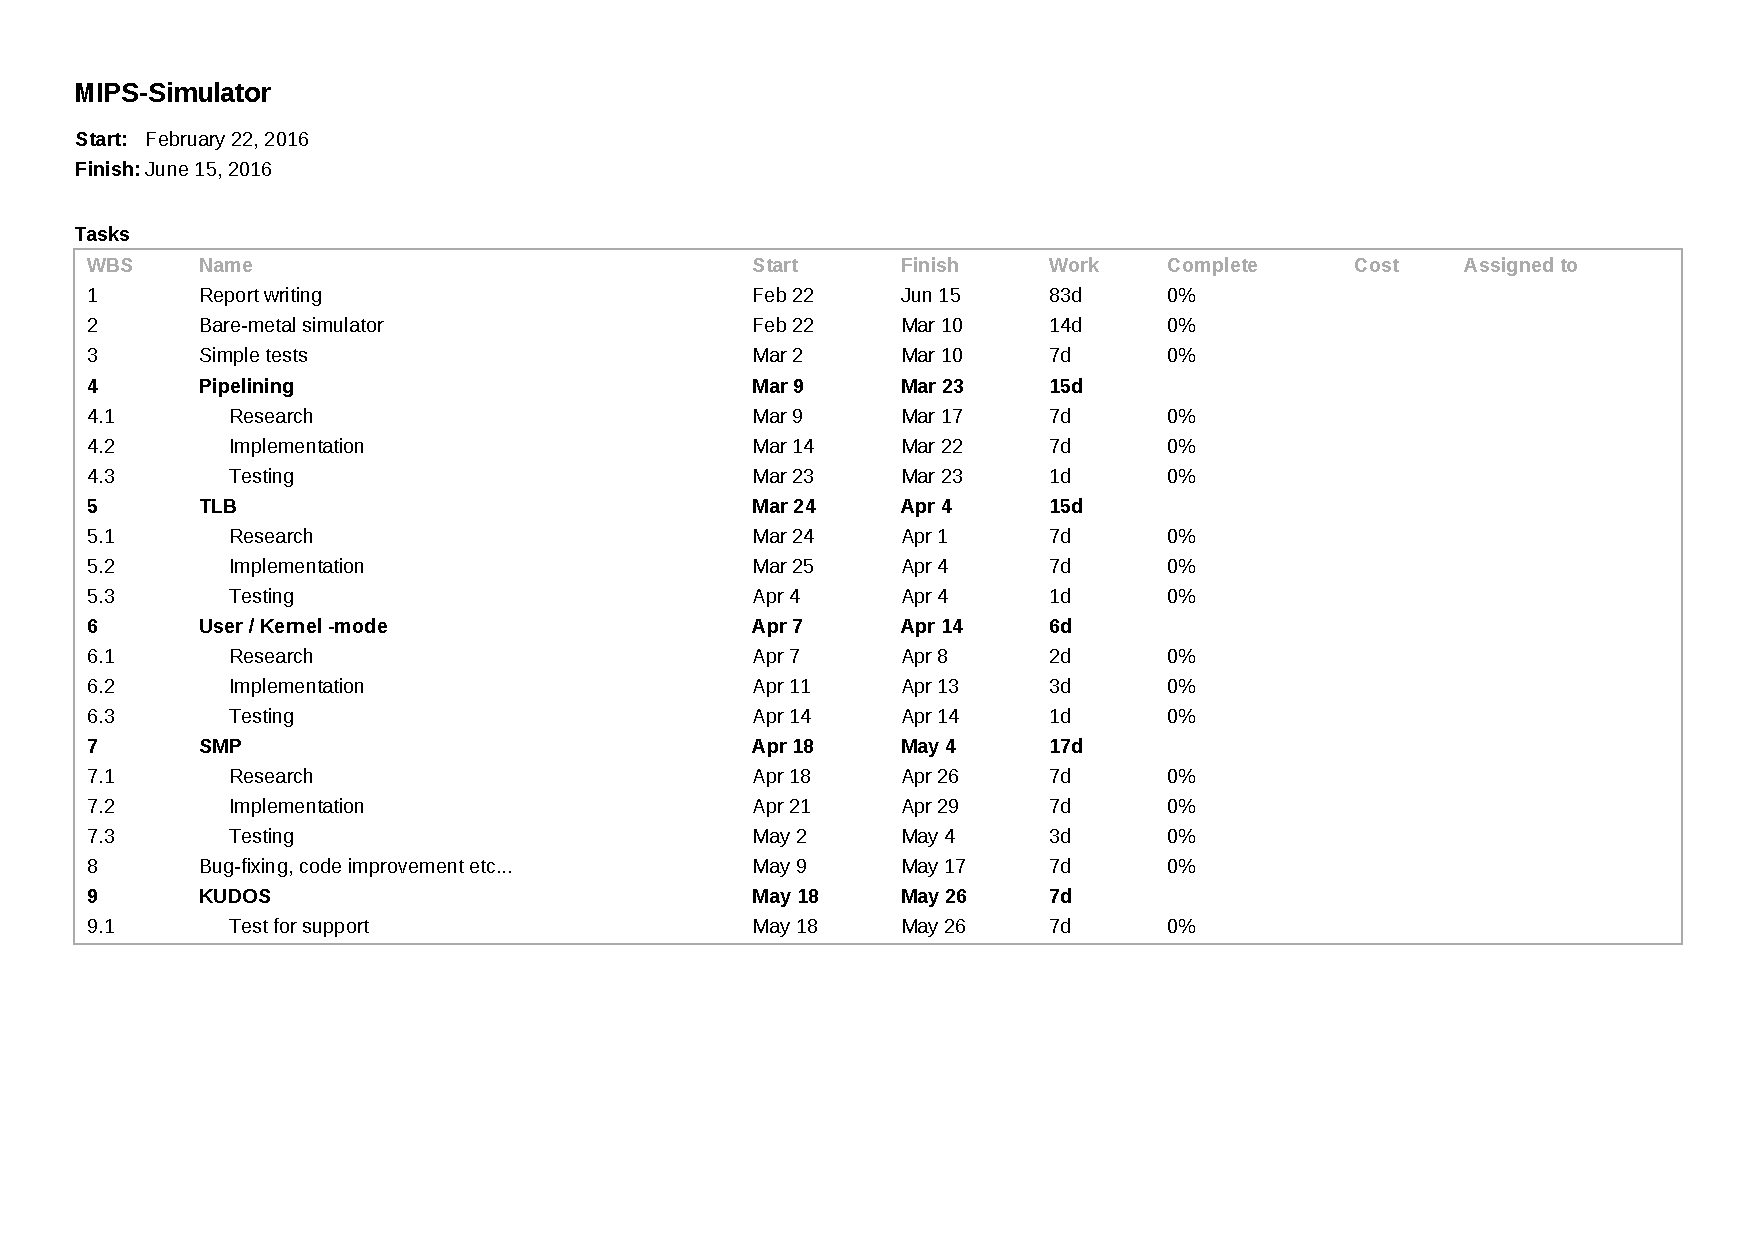
\includegraphics[scale=0.8,angle=270]{tasks.pdf}
%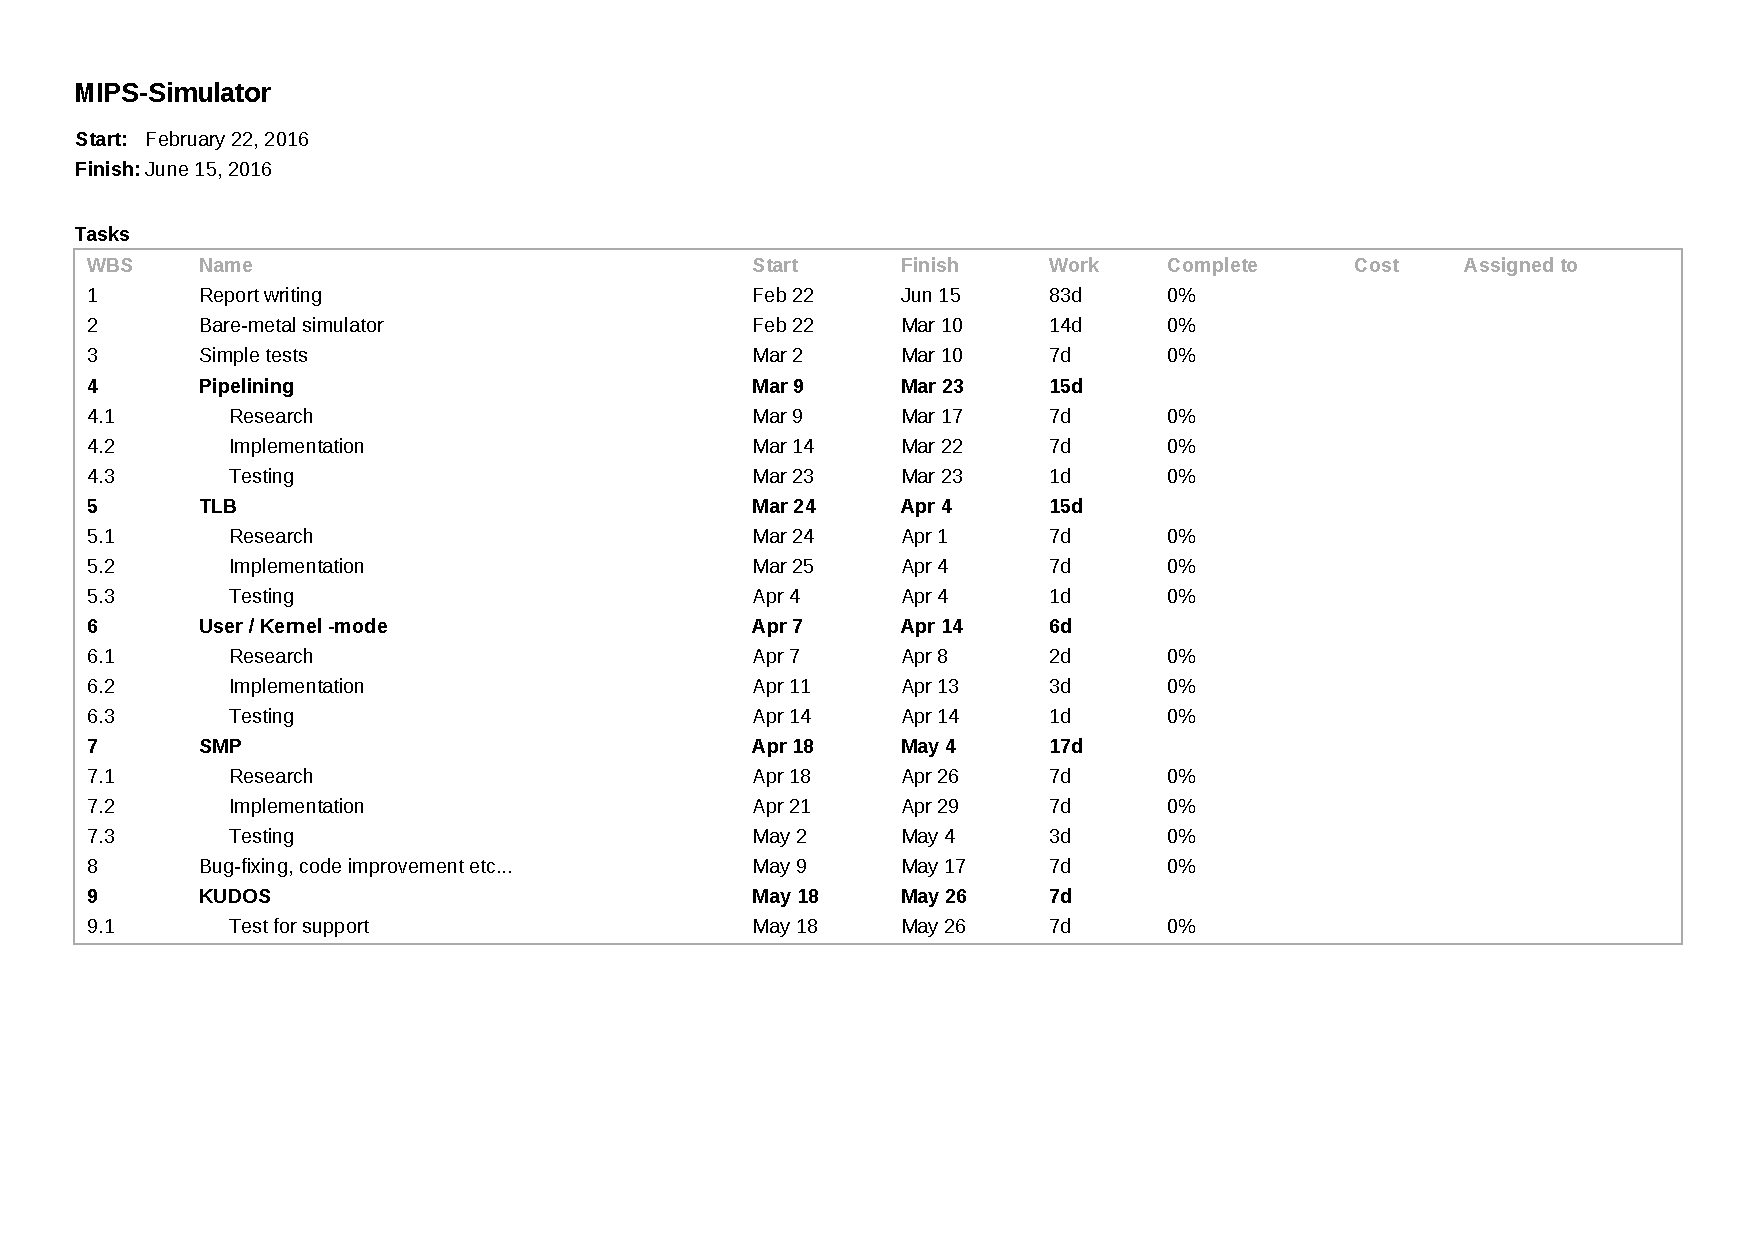
\includepdf[pages={1},angle=270,scale=0.8,pagecommand=\section{Tasks}]{tasks.pdf}
\end{appendices}

\end{document}


